\documentclass[ignorenonframetext,aspectratio=169]{beamer}
\setbeamertemplate{caption}[numbered]
\setbeamertemplate{caption label separator}{: }
\setbeamercolor{caption name}{fg=normal text.fg}
\beamertemplatenavigationsymbolsempty
\usepackage{lmodern}
\usepackage{amssymb,amsmath}
\usepackage{ifxetex,ifluatex}
\usepackage{fixltx2e} % provides \textsubscript
\ifnum 0\ifxetex 1\fi\ifluatex 1\fi=0 % if pdftex
  \usepackage[T1]{fontenc}
  \usepackage[utf8]{inputenc}
\else % if luatex or xelatex
  \ifxetex
    \usepackage{mathspec}
  \else
    \usepackage{fontspec}
  \fi
  \defaultfontfeatures{Ligatures=TeX,Scale=MatchLowercase}
\fi
% use upquote if available, for straight quotes in verbatim environments
\IfFileExists{upquote.sty}{\usepackage{upquote}}{}
% use microtype if available
\IfFileExists{microtype.sty}{%
\usepackage{microtype}
\UseMicrotypeSet[protrusion]{basicmath} % disable protrusion for tt fonts
}{}
\newif\ifbibliography
\hypersetup{
            pdfborder={0 0 0},
            breaklinks=true}
\urlstyle{same}  % don't use monospace font for urls

% Prevent slide breaks in the middle of a paragraph:
\widowpenalties 1 10000
\raggedbottom

\AtBeginPart{
  \let\insertpartnumber\relax
  \let\partname\relax
  \frame{\partpage}
}
\AtBeginSection{
  \ifbibliography
  \else
    \let\insertsectionnumber\relax
    \let\sectionname\relax
    \frame{\sectionpage}
  \fi
}
\AtBeginSubsection{
  \let\insertsubsectionnumber\relax
  \let\subsectionname\relax
  \frame{\subsectionpage}
}

\setlength{\parindent}{0pt}
\setlength{\parskip}{6pt plus 2pt minus 1pt}
\setlength{\emergencystretch}{3em}  % prevent overfull lines
\providecommand{\tightlist}{%
  \setlength{\itemsep}{0pt}\setlength{\parskip}{0pt}}
\setcounter{secnumdepth}{0}
\usepackage[default]{lato}
\pdfmapfile{=lato.map}
\usepackage[official]{eurosym}
\usepackage{booktabs}
\usepackage[makeroom]{cancel}
\usepackage{amsmath}


\setbeamertemplate{itemize subitem}{\scriptsize{$\bullet$}}


\makeatletter
\newif\if@borderstar
\def\bordermatrix{\@ifnextchar*{%
\@borderstartrue\@bordermatrix@i}{\@borderstarfalse\@bordermatrix@i*}%
}
\def\@bordermatrix@i*{\@ifnextchar[{\@bordermatrix@ii}{\@bordermatrix@ii[()]}}
\def\@bordermatrix@ii[#1]#2{%
\begingroup
\m@th\@tempdima8.75\p@\setbox\z@\vbox{%
\def\cr{\crcr\noalign{\kern 2\p@\global\let\cr\endline }}%
\ialign {$##$\hfil\kern 2\p@\kern\@tempdima & \thinspace %
\hfil $##$\hfil && \quad\hfil $##$\hfil\crcr\omit\strut %
\hfil\crcr\noalign{\kern -\baselineskip}#2\crcr\omit %
\strut\cr}}%
\setbox\tw@\vbox{\unvcopy\z@\global\setbox\@ne\lastbox}%
\setbox\tw@\hbox{\unhbox\@ne\unskip\global\setbox\@ne\lastbox}%
\setbox\tw@\hbox{%
$\kern\wd\@ne\kern -\@tempdima\left\@firstoftwo#1%
\if@borderstar\kern2pt\else\kern -\wd\@ne\fi%
\global\setbox\@ne\vbox{\box\@ne\if@borderstar\else\kern 2\p@\fi}%
\vcenter{\if@borderstar\else\kern -\ht\@ne\fi%
\unvbox\z@\kern-\if@borderstar2\fi\baselineskip}%
\if@borderstar\kern-2\@tempdima\kern2\p@\else\,\fi\right\@secondoftwo#1 $%
}\null \;\vbox{\kern\ht\@ne\box\tw@}%
\endgroup
}
\makeatother

\title{The Impact of Repossession Risk on Mortgage Default\\}
\author{Terry O'Malley\\[2\baselineskip]University College Dublin}
\date{September 05, 2018\\
EDGE 2018}

\begin{document}
\frame{\titlepage}

\section{Does reducing repossession risk lead to an increase in mortgage
default?}\label{does-reducing-repossession-risk-lead-to-an-increase-in-mortgage-default}

\begin{frame}{Repossession Risk and Mortgage Default}

\begin{itemize}
\tightlist
\item
  Moral hazard
\end{itemize}

\begin{itemize}
\tightlist
\item
  Importance of the household default cost parameter

  \begin{itemize}
  \tightlist
  \item
    Financial stability: leverage choice (Bailey et al, 2018)
  \item
    Ex-post debt renegotiation: HAMP in the US, similar programmes
    elsewhere
  \item
    Policy: foreclosure moratoria
  \end{itemize}
\item
  Strategic default

  \begin{itemize}
  \tightlist
  \item
    Are borrowers strategic when it comes to default?
  \item
    Implications for mortgage contract design
  \end{itemize}
\end{itemize}

\end{frame}

\begin{frame}{This paper}

\begin{itemize}
\item
  Exploit \emph{quasi-experimental variation in Irish repossession law}
  to test whether repossession risk matters for mortgage default.
\item
  Analyse whether \emph{treated loans defaulted at a higher rate} after
  a legal ruling striking down law.
\item
  Analyse heterogeneous treatment effects to answer: is excess default
  strategic?

  \begin{itemize}
  \tightlist
  \item
    Distressed borrower welfare enhanced?
  \item
    Or just strategic borrowers getting the benefit?
  \end{itemize}
\end{itemize}

\end{frame}

\begin{frame}{Preview of results}

\begin{itemize}
\tightlist
\item
  Methodology

  \begin{itemize}
  \tightlist
  \item
    Cut-off date in a legal judgment: law does not apply to originated
    before cut-off
  \item
    Two cohorts originated either side of the cut-off date
  \item
    Difference-in-differences research design comparing pre and post
    default rates
  \end{itemize}
\item
  Removing repossession risk lead to an immediate increase in default
  rates.

  \begin{itemize}
  \tightlist
  \item
    1-2 pp increase in cumulative default probability in one year after
    event.
  \item
    \textasciitilde{}40\% increase over estimated counterfactual.
  \end{itemize}
\item
  Treatment effect highest for loans with

  \begin{itemize}
  \tightlist
  \item
    lowest and negative home equity
  \item
    previous missed payments
  \end{itemize}
\end{itemize}

\end{frame}

\begin{frame}{What does economic theory tell us?}

\begin{itemize}
\tightlist
\item
  Reducing the cost associated with mortgage default should increase the
  demand for it.

  \begin{itemize}
  \tightlist
  \item
    Home repossession large cost of default
  \item
    Default may not be optimal
  \end{itemize}
\item
  Social theory:

  \begin{itemize}
  \tightlist
  \item
    Mortgage default isn't a rational cost-benefit calculation
  \item
    Driven by emotion, not ameniable to economic analysis
  \item
    Reduced default costs should not matter
  \end{itemize}
\item
  Not exactly clear from economic theory who excess defaulters are

  \begin{itemize}
  \tightlist
  \item
    Strategic default: inframarginal borrowers default
  \end{itemize}
\end{itemize}

\end{frame}

\begin{frame}{Economic evidence}

\begin{itemize}
\tightlist
\item
  Public finance, health: moral hazard exists

  \begin{itemize}
  \tightlist
  \item
    Einav \& Finkelstein (2018): ``compelling evidence that moral hazard
    in health insurance exists''
  \end{itemize}
\item
  Mortgage market evidence more mixed

  \begin{itemize}
  \tightlist
  \item
    Mayer et al (2014): mortgage renegotiation programme led to
    increased default rates in U.S.
  \item
    Ganong \& Noel (2017): \textbf{Low} moral-hazard cost because
    mortgage default primarily driven by affordability
  \item
    Agarwal et al (2017): No moral hazard effect from HAMP, a
    well-designed intervention
  \item
    Collins \& Urban (2016): No default response to New Jersey
    foreclosure moratorium
  \end{itemize}
\end{itemize}

\end{frame}

\section{Research Design}\label{research-design}

\begin{frame}{Ireland: 2011 Court Judgment}

\begin{itemize}
\item
  2009 Land Act

  \begin{itemize}
  \tightlist
  \item
    December 2009: Land and Conveyancing Law Reform Act replaces 1964
    law.
  \end{itemize}
\item
  July 2011: Justice Dunne rules that 2009 Act \textbf{failed to
  preserve relevant parts of the older law}
\item
  After July 2011, mortgages originated before 1st December 2009
  \emph{cannot be repossessed} if borrower defaults.

  \begin{itemize}
  \tightlist
  \item
    2 years passed before law fixed
  \end{itemize}
\end{itemize}

\end{frame}

\begin{frame}{A natural experiment}

\begin{itemize}
\tightlist
\item
  For loans originated around \emph{1st December 2009}: repossession
  risk quasi-randomly removed 1.5 years later in July 2011.

  \begin{itemize}
  \tightlist
  \item
    Treatment group originated before the cut-off
  \item
    Control group after
  \end{itemize}
\item
  Plausibly exogeneous: treatment group did not rush to get mortgages
  before the new law

  \begin{itemize}
  \tightlist
  \item
    Minor change to conveyancing law, routine procedure
  \item
    Legal ruling \emph{not anticipated}
  \end{itemize}
\item
  Difference-in-difference: use outcome of control group to estimate
  missing counterfactual for treatment group.
\end{itemize}

\end{frame}

\begin{frame}{}

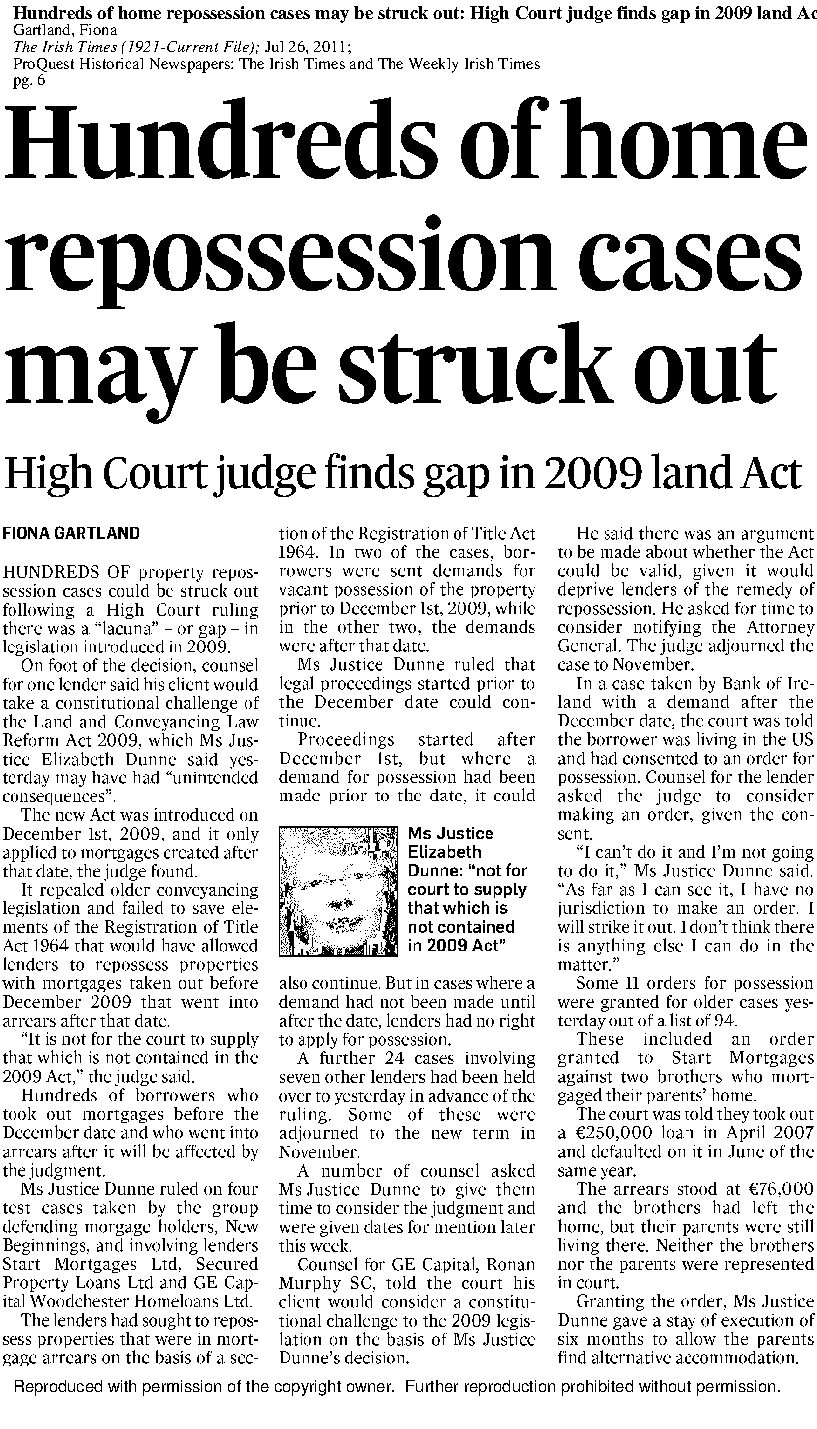
\includegraphics[width = 0.45\linewidth]{july26.pdf}
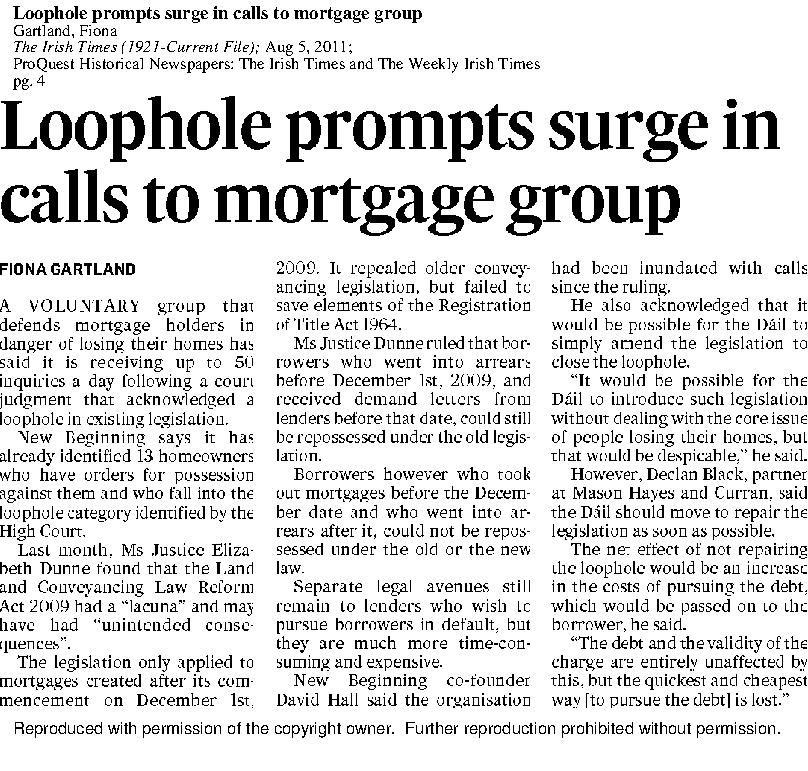
\includegraphics[width = 0.45\linewidth]{loophole.pdf}

\end{frame}

\begin{frame}{Data}

\begin{itemize}
\item
  Central Bank of Ireland Loan-Level Data
\item
  Collected from regulated banks for stress-testing, 2010-present
\item
  Quarterly panel data with information on

  \begin{itemize}
  \tightlist
  \item
    \emph{current} loan characteristics
  \item
    \emph{origination} borrower characteristics
  \end{itemize}
\end{itemize}

\end{frame}

\begin{frame}{Paper data set}

\begin{itemize}
\item
  Take loans originated 180 days before and after the cut-off date in
  legal ruling: 1st December 2009

  \begin{itemize}
  \tightlist
  \item
    Pre cut-off are the treatment group
  \end{itemize}
\item
  Q3/2010 - Q2/2012
\item
  Loans are matched by an estimated propensity score

  \begin{itemize}
  \tightlist
  \item
    Future treatment group status as a function of first period
    covariates
  \item
    Matching without replacement to eliminate observations without
    counterpart
  \end{itemize}
\item
  80,732 observations. 7,913 loans. Half treatment, half control.
\end{itemize}

\end{frame}

\begin{frame}{Mortgage default}

\[
\textup{default}{}_{it}=P(90\textup{DPD}_{it}=1\,|\,90\textup{DPD}_{is}=0\textup{\,for all }s<t)
\]

\begin{itemize}
\item
  Loan \(i\) is in default at time \(t\) if it has accumlated greater
  than 90 days worth of missed payments.
\item
  Standard Basel definition of loan default
\item
  Less noisy than using surrogate measures such as 30 days past due etc.
\item
  Loan drops out of data once in default

  \begin{itemize}
  \tightlist
  \item
    Theoretical interest is in the \emph{transition} to default and not
    the state of being in default
  \end{itemize}
\end{itemize}

\end{frame}

\begin{frame}{Difference in means}

Stock (left) v transition (right)
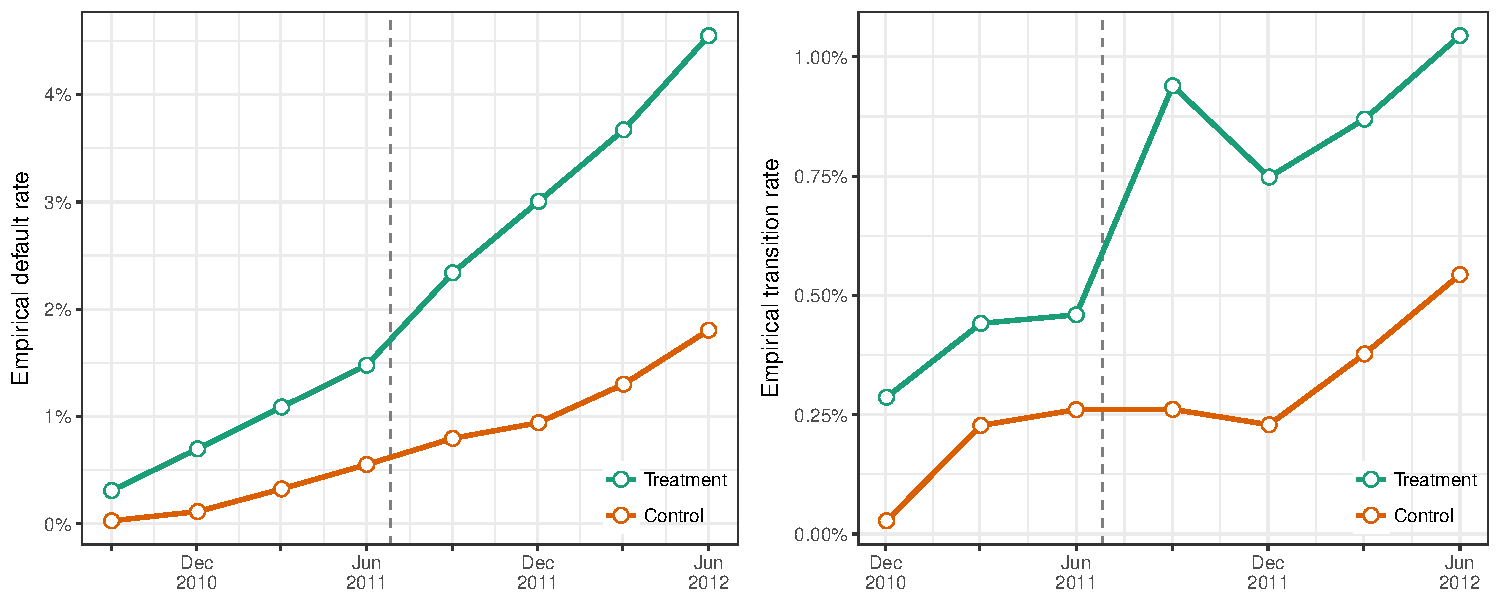
\includegraphics[width=\linewidth]{empirical_wide}

\end{frame}

\section{Estimation and Inference}\label{estimation-and-inference}

\begin{frame}{Estimating Equation}

\begin{equation}
\textup{{default}}_{ibfgrt}=\alpha+\beta^{DD}(\textup{{Treatment}}_{g}\times\textup{Post}_{t})+X_{it} +\phi_{r,t}+\tau_{b,f,t}+\epsilon_{ibfgrt}
\end{equation}

where:

\begin{itemize}
\item
  \(treatment_i\) is an indicator for whether the loan was originated
  before the cut-off.
\item
  \(Post_t\) is an indicator for whether the observation is after the
  ruling (July 2011).
\item
  \(\beta_{DD}\) is treatment effect of interest
\item
  \(X_{it}\) is a matrix of control variables including treatment
  status, interest rate, loan-to-value ratio, borrower income, borrower
  age
\item
  \(\phi_{r,t}+\tau_{b,f,t}\) are region-time and interest rate type -
  time fixed effects
\item
  Identification: within-group changes between treatment and control
  groups over time

  \begin{itemize}
  \tightlist
  \item
    Conditional on controls and fixed effects, treament \(\beta^{DD}\)
    is an unbiased estimator of treatment effect
  \end{itemize}
\item
  Inference: errors clustered at loan level.
\end{itemize}

\end{frame}

\begin{frame}{Results}

\centering
% Table created by stargazer v.5.2 by Marek Hlavac, Harvard University. E-mail: hlavac at fas.harvard.edu
% Date and time: Fri, Oct 06, 2017 - 20:00:14
\begin{tabular}{@{\extracolsep{5pt}}lccc} 
\\[-1.8ex]\hline 
\hline \\[-1.8ex] 
\\[-1.8ex] & \multicolumn{3}{c}{Default} \\ 
\\[-1.8ex] & (1) & (2) & (3)\\ 
\hline \\[-1.8ex] 
 Treatment & 0.002$^{***}$ & 0.0001 &  \\ 
  & (0.001) & (0.001) &  \\ 
  & & & \\ 
 Treatment$*$Post & 0.003$^{***}$ & 0.004$^{***}$ & 0.005$^{***}$ \\ 
  & (0.001) & (0.001) & (0.001) \\ 
  & & & \\ 
\hline \\[-1.8ex] 
Observations & 80,667 & 80,663 & 80,663 \\ 
\hline 
Time-varying controls & N & Y  & Y \\
Time FE & N & Y & -\\
Loan FE & N & N & Y \\
Region$*$RateType$*$Time FE& N & N & Y \\
\hline \\[-1.8ex] 
& \multicolumn{3}{r}{$^{*}$p$<$0.1; $^{**}$p$<$0.05; $^{***}$p$<$0.01} \\ 
\end{tabular} 


\end{frame}

\begin{frame}{Eventy study}

\begin{itemize}
\tightlist
\item
  Interact treatment dummy with time fixed effects
\end{itemize}

\footnotesize\centering
% Table created by stargazer v.5.2 by Marek Hlavac, Harvard University. E-mail: hlavac at fas.harvard.edu
% Date and time: Sat, Aug 12, 2017 - 16:51:59
\begin{tabular}{@{\extracolsep{5pt}}lc} 
& {Pre-judgment}  \\
\hline \\[-1.8ex] 
 Treatment$*$Mar-2011 &  $-$0.00003 \\ 
   & (0.001) \\ 
& \\[-1.8ex] 
 Treatment$*$Jun-2011  & 0.0003 \\ 
   & (0.001) \\ 
   & \\ 
  & {Post-judgment}  \\
  \hline \\[-1.8ex] 
Treatment$*$Sep-2011  & 0.005$^{***}$ \\ 
  & (0.002) \\ 
& \\[-1.8ex] 
Treatment$*$Dec-2011 & 0.006$^{***}$ \\ 
 & (0.002) \\ 
& \\[-1.8ex] 
Treatment$*$Mar-2012  & 0.005$^{***}$ \\ 
   & (0.002) \\ 
   & \\[-1.8ex] 
Treatment$*$Jun-2012  & 0.006$^{***}$ \\ 
  & (0.002) \\ 
   & \\ 
\hline \\[-1.8ex] 
% Observations & 80,667 & 80,663 \\ 
% \hline 
% Time-varying 
% controls & N & Y \\
% Time FE & Y & Y \\
% Loan FE & Y & Y\\
% Bank$*$RateType$*$Time FE  & N & Y \\
% Region$*$Time FE & N & Y \\

% \hline \\[-1.8ex] 
 % & \multicolumn{2}{r}{$^{*}$p$<$0.1; $^{**}$p$<$0.05; $^{***}$p$<$0.01} \\ 
\end{tabular} 


\end{frame}

\begin{frame}{Tricky inference}

\begin{itemize}
\item
  Issue: quasi-randomisation at group level
\item
  Two groups: originated pre and post 1st December 2009
\item
  Errors correlated within group? Effective sample size of 2
\end{itemize}

\(\implies\) Permutation inference

\end{frame}

\begin{frame}{Permutation Inference}

\begin{itemize}
\item
  Permutation inference aka randomisation inference
\item
  Fisher (1936); Computing power has seen resurgence (Efron \& Hastie,
  2017)
\item
  ``Permute'' the treatment vector many times and calculate your test
  statistic

  \begin{itemize}
  \tightlist
  \item
    Effect of ``true'' treatment vector should lie in the tails
  \item
    Easy to calculate an exact \(p\)-value to test null
  \end{itemize}
\item
  Intuition: if there is nothing going on, your test statistic should be
  similar to a vector of random treatments
\end{itemize}

\end{frame}

\begin{frame}{How to permute a natural experiment?}

\begin{itemize}
\item
  This natural experiment: treatment based on cut-off date
\item
  Idea: permute the cut-off date and perform the analysis exactly as
  before

  \begin{itemize}
  \tightlist
  \item
    Extract data, match with PSM, event study regression
  \end{itemize}
\item
  1000 random dates; \emph{save} treatment effects
\item
  Compare ``true'' treatment effect to the distribution of permuted ones

  \begin{itemize}
  \tightlist
  \item
    Similar to Ganong and Jaeger (2017) on Regression Kink Design
  \end{itemize}
\item
  Estimated difference could just be a fluke due to the particular
  cut-off date

  \begin{itemize}
  \tightlist
  \item
    So try \emph{many} cut-off dates
  \end{itemize}
\end{itemize}

\end{frame}

\begin{frame}{}

\centering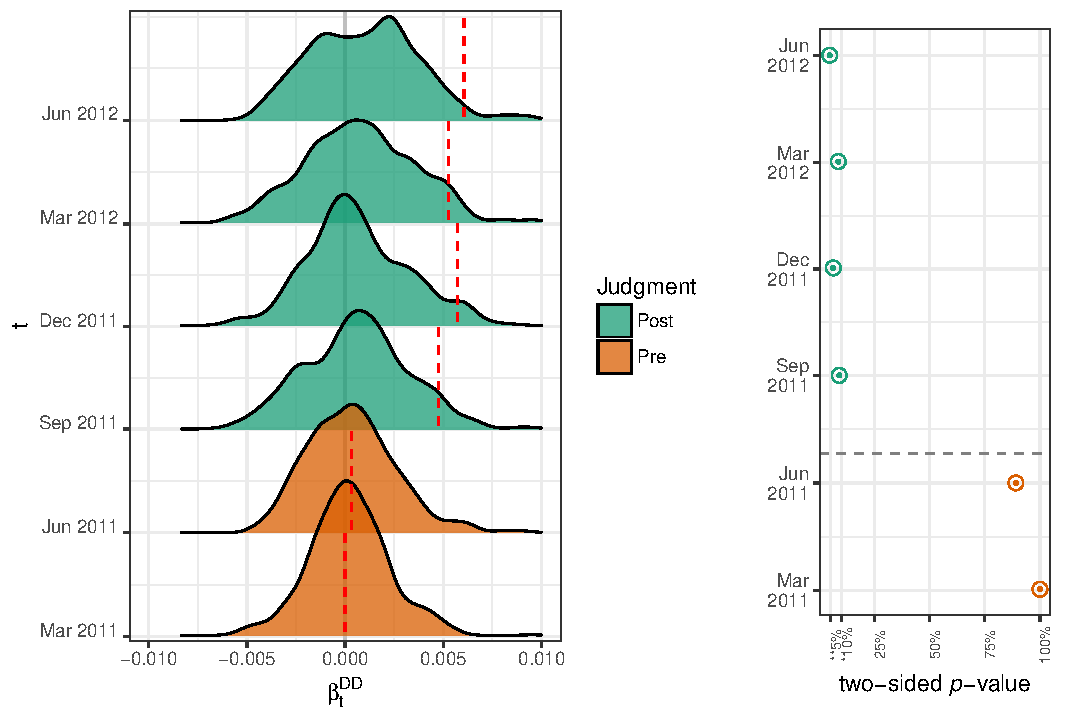
\includegraphics[width = 0.8\linewidth]{joy_with_p}

\end{frame}

\section{Heterogeneous treatment
effects}\label{heterogeneous-treatment-effects}

\begin{frame}{Beyond the avearage treatment effect}

\begin{itemize}
\item
  Average treatment effect is interesting
\item
  Is the effect driven by strategic borrowers? Or distressed borrowers?
\item
  Welfare implications of ex-post mortgage contract policies
\end{itemize}

\end{frame}

\begin{frame}{Triple difference regression}

\begin{itemize}
\item
  Effect mostly driven by households carrying a missed payment
\item
  Much smaller effect for fully-peforming households
\end{itemize}

\tiny\centering
% Table created by stargazer v.5.2 by Marek Hlavac, Harvard University. E-mail: hlavac at fas.harvard.edu
% Date and time: Mon, Jul 31, 2017 - 12:00:30
\begin{tabular}{@{\extracolsep{5pt}}lc} 
\\[-1.8ex]\hline 
\hline \\[-1.8ex] 
\\[-1.8ex] & Default \\ 
\hline \\[-1.8ex]
  &  \\  
 & Pre-judgment   \\
\hline \\[-1.8ex] 
  Treatment$*$Jun-2011 & 0.0001 \\ 
  & (0.001) \\ 
    Treatment$*$Jun-2011$*$Arrears & $-$0.0001 \\ 
	  & (0.015) \\ 
	    &  \\ 
	   & Post-judgment   \\
\hline \\[-1.8ex] 
  Treatment$*$Sep-2011 & 0.001 \\ 
  & (0.001) \\ 
  Treatment$*$Dec-2011 & 0.002$^{**}$ \\ 
  & (0.001) \\ 
  Treatment$*$Mar-2012 & 0.002$^{*}$ \\ 
  & (0.001) \\ 
  Treatment$*$Jun-2012 & 0.003$^{**}$ \\ 
  & (0.001) \\ 


  Treatment$*$Sep-2011$*$Arrears & 0.081$^{***}$ \\ 
  & (0.015) \\ 
  Treatment$*$Dec-2011$*$Arrears & 0.028$^{*}$ \\ 
  & (0.015) \\ 
  Treatment$*$Mar-2012$*$Arrears & 0.058$^{***}$ \\ 
  & (0.016) \\ 
  Treatment$*$Jun-2012$*$Arrears & $-$0.016 \\ 
  & (0.016) \\ 
% \hline \\[-1.8ex] 
%Observations & 71,240 \\ 
%\hline 
%Time-varying 
%controls & Y \\
%Loan FE & Y\\
%Time FE & Y \\
%Bank$*$Time FE & Y \\
%Region$*$Time FE & Y \\
%\hline \\[-1.8ex] 
% & \multicolumn{1}{r}{$^{*}$p$<$0.1; $^{**}$p$<$0.05; $^{***}$p$<$0.01} \\ 
\end{tabular} 


\end{frame}

\begin{frame}[fragile]{Causal forest}

\begin{quote}
Uses a random forest to reduce the curse of dimensionality in a
k-nearest neighbour estimation problem
\end{quote}

\begin{itemize}
\item
  Intuition: I want to group treatment and control observations on
  different dimensions and compare the difference in treatment effects
  across these groups - Not obvious what variables to group on and what
  intervals to use

\begin{verbatim}
<!-- - Income one of many possible variables -->
<!-- - Theory does not make it clear  -->
<!-- - Where to split high v low income -->
\end{verbatim}
\item
  You could use a kernel regression to do it but quickly run into curse
  of dimensionality 
\item
  Causal forest model uses random forest to decide how to weight nearby
  observations in a kernel regression
\end{itemize}

\end{frame}

\begin{frame}{Treatment effect function}

\begin{equation}
Y_{i}=(Y_{i1}-Y_{i0})=\tau(X_{i0},\,Z_{i1})+\epsilon_{i}\label{eq:tau}
\end{equation}

\begin{itemize}
\tightlist
\item
  Loan-level treatment effect is the difference in potential outcomes
\item
  Model how each individuals treatment effect varies according to
  covarites
\item
  2 matrices: \(X\) and \(Z\)
\item
  Panel data collapsed: endline Y as a function of pre-treatment
  covariates
\end{itemize}

\end{frame}

\begin{frame}{Predicted treatment effect of loan-to-value ratio}

Highly leveraged borrowers have lowest opportunity cost of defaulting

\centering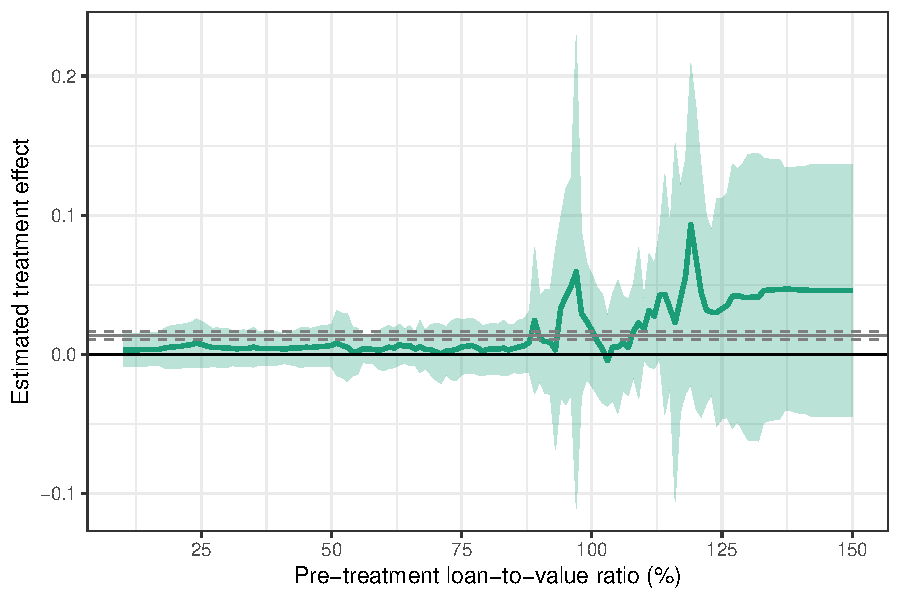
\includegraphics[width = 0.7\linewidth]{ltv_te}

\end{frame}

\begin{frame}{How are covariates associated with individual treatment
effect?}

\centering

\begin{tabular}{@{\extracolsep{5pt}}lc}
 & \tabularnewline
 & \tabularnewline
\hline 
 & \tabularnewline
 & Treatment effect\tabularnewline
\hline & \tabularnewline
LTV  & 0.0002$^{***}$ \tabularnewline
 & (0.00001) \tabularnewline
log(Income)  & $-$0.002$^{*}$ \tabularnewline
 & (0.001) \tabularnewline
Interest rate  & 0.002$^{**}$ \tabularnewline
 & (0.001) \tabularnewline
Year of birth  & $-$0.00001 \tabularnewline
 & (0.00004) \tabularnewline
Constant  & 0.027 \tabularnewline
 & (0.088) \tabularnewline
\hline & \tabularnewline
Observations  & 12,298 \tabularnewline
\hline\hline & \tabularnewline
 & \multicolumn{1}{r}{$^{*}$p$<$0.1; $^{**}$p$<$0.05; $^{***}$p$<$0.01}\tabularnewline
\end{tabular}

\end{frame}

\begin{frame}{Conclusion}

\begin{itemize}
\item
  Quasi-experimental evidence of moral hazard in the mortgage market
\item
  Between 1 and 2 pp one-year difference in default probability
\item
  Doesn't look like \emph{strategic default}

  \begin{itemize}
  \tightlist
  \item
    Excess defaults made up mostly of loans in arrears
  \item
    Causal forest reveals lower income, higher leverage, higher interest
    rate associated with high treatement effect
  \item
    Marginal not inframarginal borrowers default after the ruling
  \end{itemize}
\item
  Policy implications: reducing repossession risk as a social insurance
  programme?

  \begin{itemize}
  \tightlist
  \item
    Of course other costs: transfers default cost from borrower to bank
  \item
    Other GE effects: risk pricing, banking losses
  \end{itemize}
\end{itemize}

\end{frame}

\end{document}
